% Diese Zeile bitte -nicht- aendern.
\documentclass[course=erap]{aspdoc}

%%%%%%%%%%%%%%%%%%%%%%%%%%%%%%%%%
\newcommand{\theGroup}{110}
\newcommand{\theNumber}{A201}
\author{Simon Bußmann \and Nico Lintner \and Manuel Walter Mußbacher}
\date{Sommersemester 2023}
%%%%%%%%%%%%%%%%%%%%%%%%%%%%%%%%%

% Diese Zeile bitte -nicht- aendern.
\title{Gruppe \theGroup{} -- Abgabe zu Aufgabe \theNumber}

\usepackage{caption}
\usepackage{subcaption}

\begin{document}
\maketitle

\section{Einleitung}
\label{sec:einleitung}
In diesem Projekt haben wir uns damit beschäftigt, den Sobel-Filter Algorithmus zu implementieren.
Dieser Algorithmus wird verwendet, um Kanten in Bildern zu erkennen und findet beispielsweise Anwendung in der Bildverarbeitung und -analyse, sowie in Computer-Vision.
So kann er z.B.\ in der Medizin eingesetzt werden, um Tumore in MRT-Bildern besser erkennbar zu machen\cite{7002427},
oder in der Forensik um Fingerabdruckerkennung zu verbessern\cite{6900702}.
Als Eingabe für den Sobel-Filter wird ein 24-Bit BMP-Bild erwartet.
Jeder Pixel in einem Bild wird dabei durch drei Bytes repräsentiert, die die Farbwerte für Blau, Grün und Rot enthalten.

\subsection{Mathematische Definition des Sobel-Filters}
\label{subsec:math-def}
Der Sobel-Filter besteht daraus, die beiden Filtermatritzen $M^{v}$ und $M^{h}$ für vertikale und horizontale Kanten mit jedem Pixel des Bildes zu verrechnen.
\begin{equation}
    M^{v} :
    \begin{bmatrix}
        1 & 0 & -1
        2 & 0 & -2
        1 & 0 & -1
    \end{bmatrix}
    M^{h} :
    \begin{bmatrix}
        1 & 2 & 1
        0 & 0 & 0
        -1 & -2 & -1
    \end{bmatrix}\label{eq:mvmh}
\end{equation}
\begin{equation}
    A^{h} = M^{h} * Image\label{eq:faltenhorizontal}
\end{equation}
\begin{equation}
    A^{v} = M^{v} * Image\label{eq:faltenvertikal}
\end{equation}
Für Kantenerkennung macht es nur Sinn, die drei Farbkanäle F eines jeden Pixels mit Koordinaten (x, y) im Eingabebild B separat zu betrachten.
Um die Farbinformationen eines Pixels an Stelle x und y der vertikalen und horizontalen Kanten A zu berechnen, wird der entsprechende Farbkanal jedes umittelbar umliegenden Pixels in B mit dem dazugehörigen Wert der Filtermatritzen (M\textsuperscript{v} und M\textsuperscript{h} respektive) multipliziert und die Produkte anschließend aufsummiert.
Sollte diese Berechnung nicht möglich sein, weil sich einer der umliegenden Pixel am Rand des Bildes befindet, wird der Wert dieses Farbwerts (und damit implizit auch der Wert des gesamten Pixels) im Ausgabebild als 0 (schwarz) angenommen.
Dadurch ergibt sich ein impliziter schwarzer Rand im Ausgabebild.
\begin{equation}
    A_(x,y)^{v,F} = \sum_{i=-1}^{1} \sum_{j=-1}^{1} M^{v}_{i,j} * B_{(x+i,y+j)}^{F}\label{eq:sumav}
\end{equation}
\begin{equation}
    A_(x,y)^{h,F} = \sum_{i=-1}^{1} \sum_{j=-1}^{1} M^{h}_{i,j} * B_{(x+i,y+j)}^{F}\label{eq:sumah}
\end{equation}
Um letztendlich den konkreten Sobelwert für einen Pixel zu berechnen, wird der Satz des Pythagoras auf die Ergebnisse der beiden vorherigen Gleichungen angewendet.
\begin{equation}
    O^{F}_{x,y} = \sqrt{(A^{v,F}_{x,y})^2 + (A^{h,F}_{x,y})^2}
    \label{eq:wurzel}
\end{equation}
Die hieraus resultierenden Werte werden dann in einem neuen Bild O gespeichert.
\begin{figure}[H]
    \begin{subfigure}{.5\columnwidth}
        \centering
        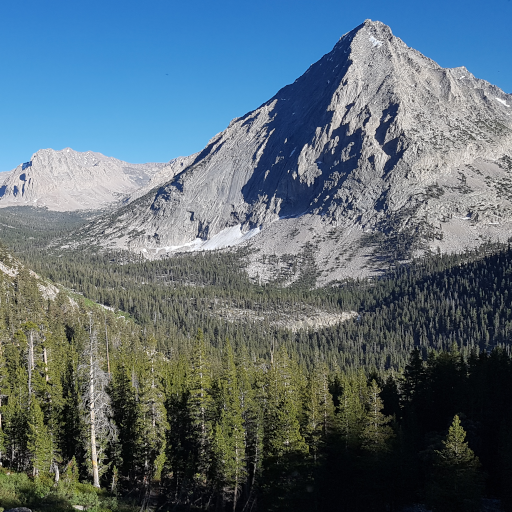
\includegraphics[width=\columnwidth]{graphics/johnmuirtrail}
        \caption{Input-Bild}
        \label{fig:input-bild}
    \end{subfigure}
    \begin{subfigure}{.5\columnwidth}
        \centering
        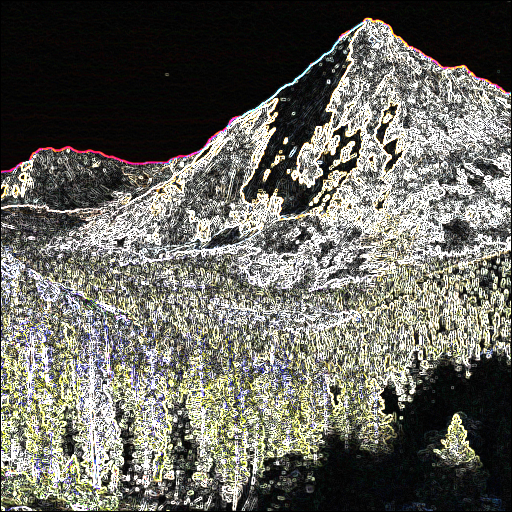
\includegraphics[width=\columnwidth]{graphics/johnmuirtrail_sobel}
        \caption{Output-Bild}
        \label{fig:output-bild}
    \end{subfigure}
\end{figure}

Abbildung \ref{fig:input-bild} und \ref{fig:output-bild} zeigen ein Input-Bild und das Resultat, das (unsere) Sobel-Implementierung produziert.
Es fällt auf, dass sehr viele Kanten im Resultat eine prägnante Farbe haben.
Da diese Farbe für Kantenerkennung üblicherweise weniger interessant ist, wird der Sobel-Filter in der Regel auf Graustufenbildern angewendet, wodurch alle Kanten weiß und die übrigen Pixel schwarz werden.

\section{Lösungsansatz}\label{sec:losungsansatz}
Unser gewählter Lösungsansatz besteht aus drei verschiedenen Versionen:
Die Basisversion (Version 0) übersetzt die mathematische Definition des Sobel-Filters aus \ref{subsec:math-def} schlicht in C-Code (mit einer kleinen Anpassung, siehe \ref{subsec:vergleichsimplementierung}).
Um diese Version als verlässliche Vergleichsimplementierung verwenden zu können, ist sie so einfach und leserlich wie möglich.

Version Eins und Zwei bauen jeweils aufeinander auf und zielen darauf ab, die Laufzeit der Basisversion bedeutend zu verbessern:
Version Eins verwendet dafür Single Instruction Multiple Data (SIMD) Instruktionen, um eine größere Bandbreite bei der Berechnung des Filters zu erreichen.
Dabei werden die Farbwerte von mehr als 5 Pixeln simultan berechnet und gespeichert.
Version Zwei kombiniert besagte erhöhte Bandbreite mit Multithreading, um die hohe Parallelität moderner Prozessoren optimal auszunutzen.

Jede der drei Versionen hat ein Gegenstück (Version 3 - Version 5 respektive), das mit Graustufenbildern (8-Bit BMPs) arbeitet.
Diese Versionen sind für diesen Teil nicht weiter interessant, da sie exakt dieselbe Funktionsweise haben und sich lediglich in der Anzahl der Bits pro Pixel, nämlich 8 statt 24, unterscheiden - wodurch sich natürlich auch die Anzahl der nötigen Berechnungen um Faktor 3 reduziert.

\subsection{Vergleichsimplementierung - Version 0}
\label{subsec:vergleichsimplementierung}
Die Vergleichsimplementierung ist eine naive Implementierung des Sobel-Filter Algorithmus und orientiert sich, wie bereits erwähnt, sehr stark an der mathematischen Definition aus \ref{subsec:math-def}.
Um diese Version auch tatsächlich als Vergleich zu den Optimierungen verwenden zu können, verwendet sie jedoch eine Annäherung an den Satz des Pythagoras \ref{eq:wurzel}.
Dafür wird, statt die Wurzel aus der Summe der Quadrate zu ziehen, die Summe der Absolutbeträge berechnet.

\begin{equation}
    O^{F}_{x,y} = \left | A^{v,F}_{x,y} \right | + \left | A^{h,F}_{x,y} \right |
    \label{eq:betrag}
\end{equation}

Dies hat den einfach Grund, dass keine SIMD-Instruktion zur (effizienten) Berechnung der Wurzel aus (16-Bit) Ganzzahlen im SSE4.2-Instruktionssatz existiert.
\begin{figure}[H]
    \begin{subfigure}{.5\columnwidth}
        \centering
        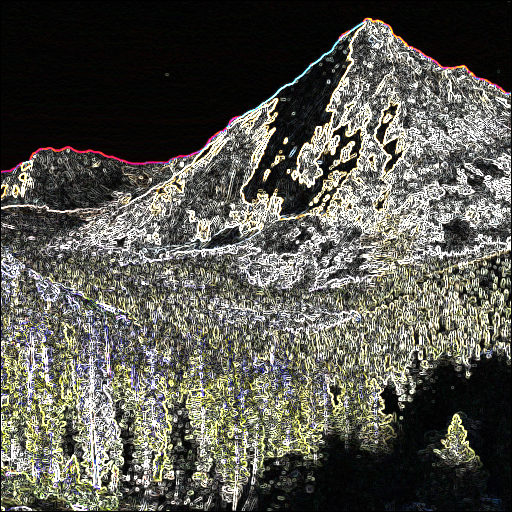
\includegraphics[width=\columnwidth]{graphics/sqrt_sobel}
        \caption{Pythagoras\ref{eq:wurzel}}
        \label{fig:sqrt-bild}
    \end{subfigure}
    \begin{subfigure}{.5\columnwidth}
        \centering
        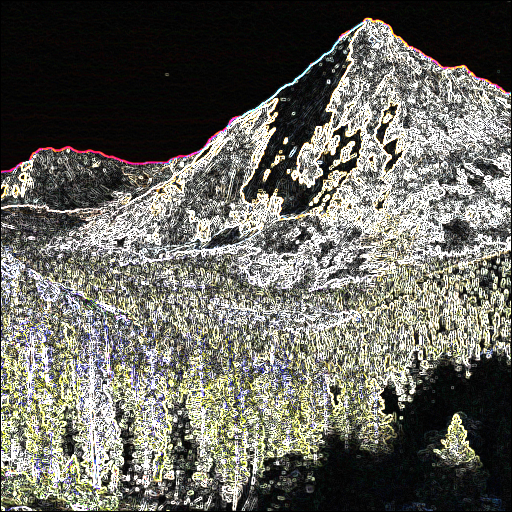
\includegraphics[width=\columnwidth]{graphics/johnmuirtrail_sobel}
        \caption{Annäherung\ref{eq:betrag}}
        \label{fig:abs-bild}
    \end{subfigure}
\end{figure}
Der Unterschied zwischen \ref{fig:abs-bild} und \ref{fig:sqrt-bild} ist marginal und liegt lediglich in der Helligkeit des Bildes, was für Kantenerkennung in diesem Ausmaß vernachlässigbar ist.
\subsection{SIMD Implementierung - Version 1}
\label{subsec:simd-implementierung}
Die SIMD Implementierung basiert algorithmisch auf der Vergleichsimplementierung, benutzt zur Berechnung jedoch SIMD Instruktionen und optimiert Speicherzugriffe.
Ein großes Problem bei der Arbeit mit 8-Bit-Ganzzahlen ist der kleine Wertebereich.
Da die Werte der einzelnen Farbchannel der Pixel als 8 Bit Integer gespeichert werden, kann es sehr schnell zu einem Überlauf kommen.
Der naive Lösungsansatz, um dem entgegen zu wirken, ist, das Input-Bild schlicht um 75\% zu verdunkeln. \label{sec:verdunkeln}
Durch die Verdunkelung wird der Überlauf zwar verhindert, das Resultat ist jedoch (wesentlich) dunkler {\ref{fig:dark}}, wodurch auch die erkannten Kanten signifikant dunkler werden.
\begin{figure}[H]
    \begin{subfigure}{.5\columnwidth}
        \centering
        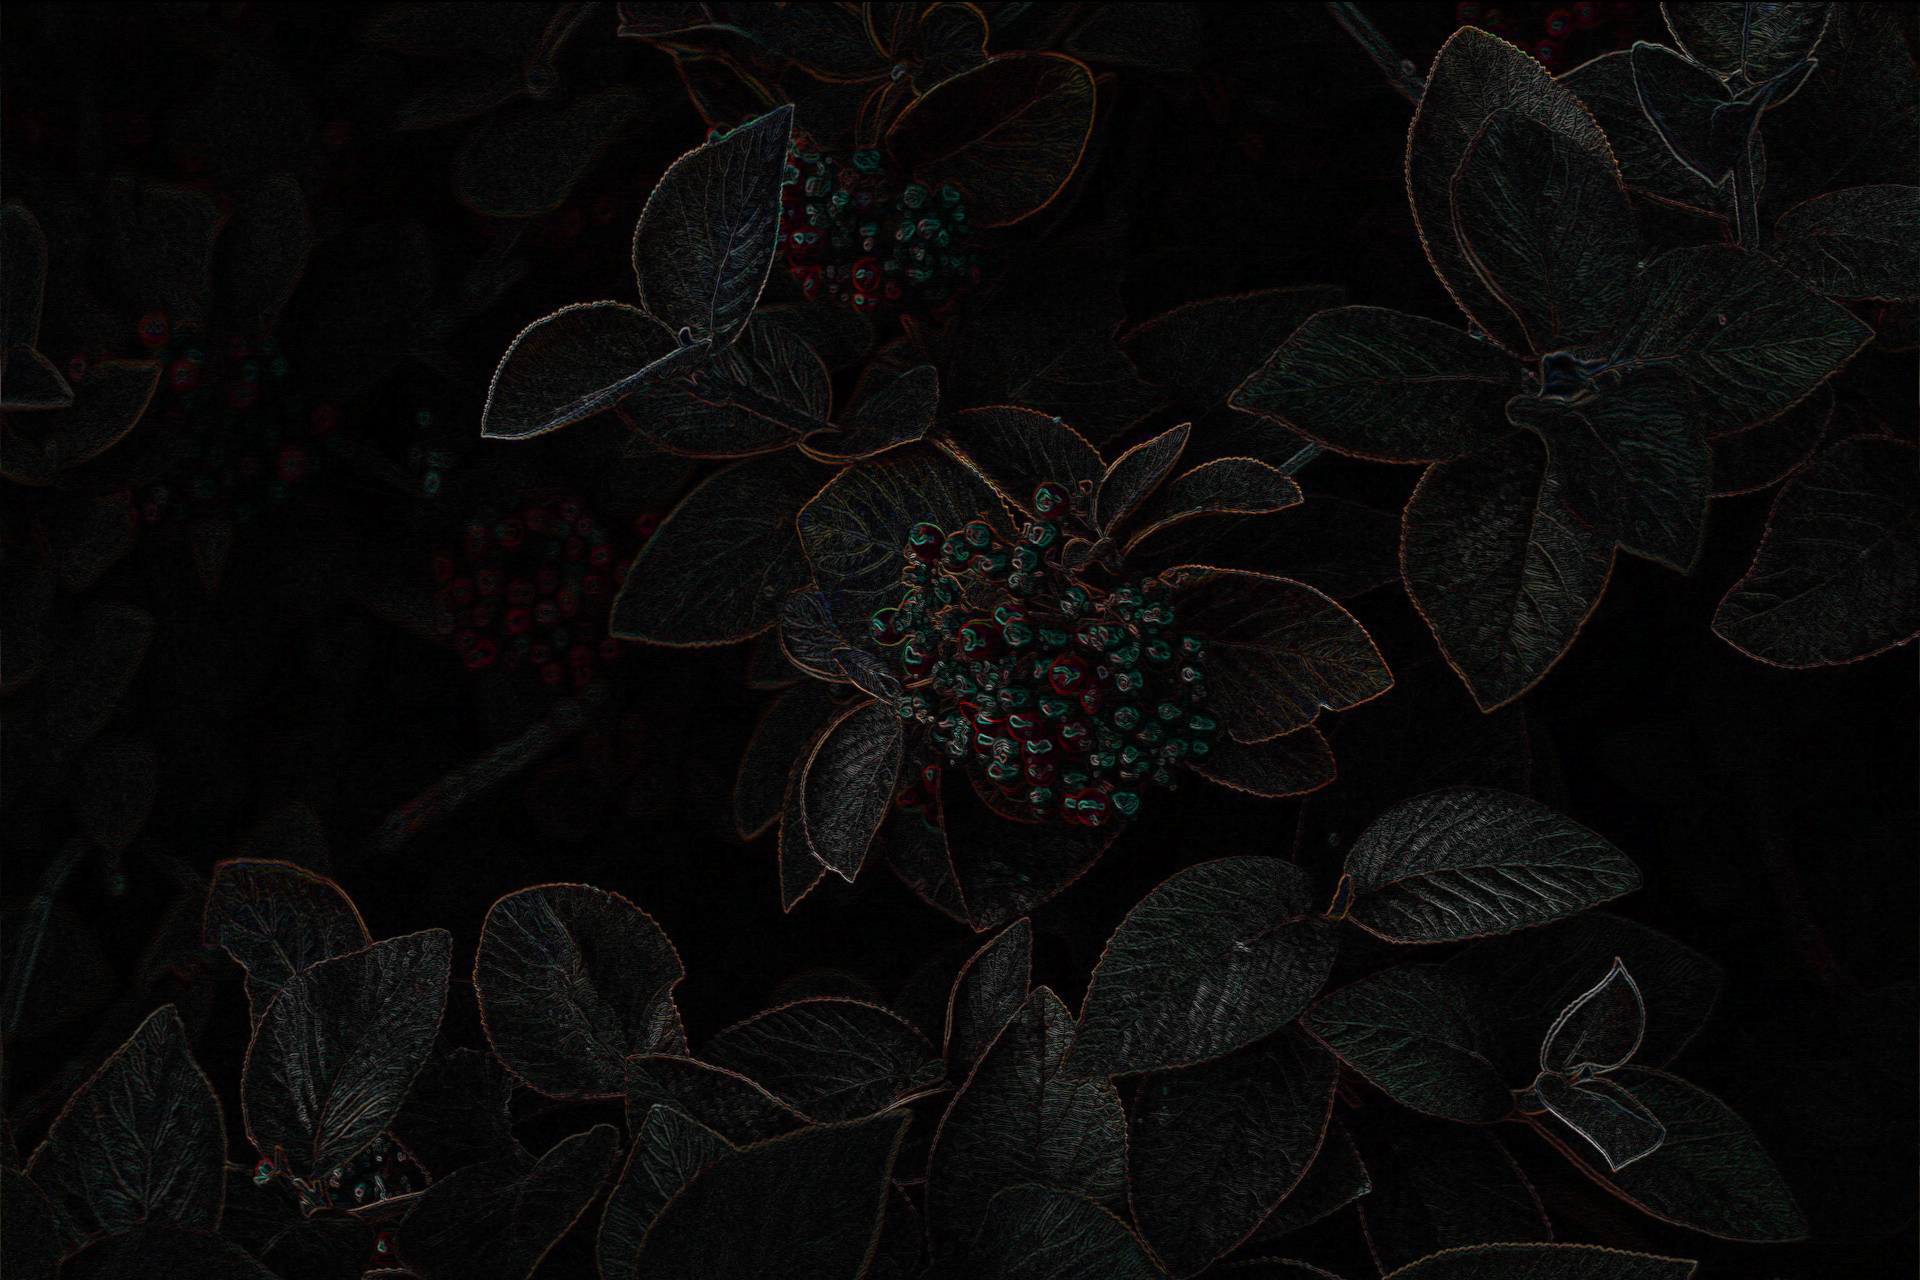
\includegraphics[width=\columnwidth]{graphics/dark}
        \caption{naiver SIMD Ansatz\ref{sec:verdunkeln}}
        \label{fig:dark}
    \end{subfigure}
    \begin{subfigure}{.5\columnwidth}
        \centering
        \includegraphics[width=\columnwidth]{graphics/correct}
        \caption{Vergleichsimplementierung\ref{subsec:vergleichsimplementierung}}
        \label{fig:correct}
    \end{subfigure}
\end{figure}
Um trotz Vektorinstruktionen und sehr kleinen Wertebereichen ein Ergebnis zu erzielen,
das exakt der Vergleichsimplementierung entspricht, werden die Daten aus einem 16-Byte-Speicherbereich so in zwei Vektoren geladen, dass während der Berechnung je 8 Byte
als 16-Bit-Integer interpretiert werden können.
Dabei werden insgesamt 16 Vektoren genutzt, um die Sobel Werte für 16 Farbchannel gleichzeitig zu berechnen.
Das funktioniert so, dass ein 16 Byte-Speicherbereich gelesen wird und anschließend das jeweils höherwertige Byte eines jeden
16-Bit-Integers in diesem Vektor mit einer Bitmaske genullt wird.
Das geschieht analog mit den 16-Byte an der um einen Byte höheren Speicheradresse, wodruch danach alle 16 Bytes der Speicheradresse in zwei Vektoren verteilt liegen.
Für jeden der 16 Farbchannel, die mit einem Schleifendurchlauf berechnet werden können, werden so die acht umliegenden entsprechenden Farbchannel geladen.
Durch den entstehenden Overhead ist dieser Lösungsansatz zwar ca.\ nur halb so schnell, wie der naive SIMD-Ansatz, erzeugt jedoch ein korrektes Ergebnis, weshalb das Programm auch diesen Ansatz implementiert.

\subsection{SIMD-Implementierung mit Threading - Version 2}
\label{subsec:simd-threading}
Die SIMD-Implementierung mit Threading basiert auf der SIMD-Implementierung mit der Besonderheit, dass das Bild in Abschnitte eingeteilt wird, die jeweils von einem eigenen Thread bearbeitet werden.
Um diese Abschnitte zu erzeugen, wird das Bild in horizontale Streifen geschnitten.
Die Anzahl der Streifen wird von der Anzahl der durch die CPU bereitgestellten Threads bestimmt, was auf eine optimale Nutzung der zur Verfügung stehenden Ressourcen abzielt.
Das horizontale Zerteilen des Bildes hat gleich mehrere Vorteile:
Der wohl größte Vorteil ist, dass das Cacheverhalten sehr viel besser ist, als es das zum Beispiel beim Aufteilen in vertikale Streifen wäre, da die Daten hintereinander, Zeile für Zeile, im Speicher liegen.
Außerdem bietet es sich sehr gut an, die Anzahl der Streifen dynamisch zu berechnen, wodurch ein System mit mehr Ressourcen besser ausgelastet werden kann.
Ein weiterer Vorteil besteht darin, fortlaufende Indizes bei der Berechnung nutzen zu können und nicht, wie zum Beispiel bei einer Aufteilung in Quadranten, diese Indizes aufwendig berechenen zu müssen.
Zuletzt lässt sich noch argumentieren, dass auch die Berechnung der Streifen selbst sehr schnell ausführbar ist, da nur eine Division benötigt wird.
Beispielsweise würde somit ein Bild mit den Dimensionen 1920x1080 (Full-HD), auf einer CPU mit 4 Threads, in 4 Streifen mit den Dimensionen 1920x270 aufgeteilt und auf 4 POSIX-Threads verteilt werden.

\section{Genauigkeit}\label{sec:genauigkeit}
Im folgenden wird die Genauigkeit unseres Lösungsansatzes analysiert, da es beim Sobel Operator keine fest definierte \enquote{source of truth}, wie zum Beispiel bei einer Addition, gibt.
Die öffentlich existierende Sobel-Filter Implementierung von OpenCV liefert beispielsweise Ergebnisse, die sich leicht in der Helligkeit von unserer unterscheiden.
Desweiteren arbeitet diese auf Graustufenbildern, wohingegen unsere Implementierung auf RGB-Bildern arbeitet.
Wir haben die Implementierung von OpenCV so angepasst, dass sie ebenfalls auf RGB-Bildern arbeiten kann, um die Ergebnisse mit unseren zu vergleichen.
\begin{figure}[H]
    \begin{subfigure}{.5\columnwidth}
        \centering
        \includegraphics[width=\columnwidth]{graphics/basic}
        \caption{Vergleichsimplementierung}
        \label{fig:basic}
    \end{subfigure}
    \begin{subfigure}{.5\columnwidth}
        \centering
        \includegraphics[width=\columnwidth]{graphics/open_cv}
        \caption{Open CV Version}
        \label{fig:opencv}
    \end{subfigure}
\end{figure}
In \ref{fig:basic} ist die Vergleichsimplementierung zu sehen, in \ref{fig:opencv} die OpenCV Implementierung.
Es ist zu erkennen, dass die OpenCV Implementierung anders belichtet erscheint, als das Resultat unserer Basisversion, was auf die automatische Anwendung von Noise-bereinigenden Filtern zurückzuführen sein dürfte.
Da die Kanten dennoch korrekt (!und kontrastreicher!) erkannt werden, und um überflüssige Rechenschritte zu vermeiden, wird das Ergebnis der Vergleichsimplementierung nicht weiter angepasst.

Bei der weiteren Bewertung der Genauigkeit wird die Vergleichsimplementierung als Referenzpunkt verwendet.
Sie gilt als das korrekte Ergebnis und ist, um Fehler zu vermeiden, so simpel und leserlich gehalten wie nur irgendwie möglich.
Da die mathematische Defintion, wie in \ref{subsec:vergleichsimplementierung} beschrieben, ohne weitere Optimierungen umgesetzt wurde, ist deren Übereinstimmung unschwer zu überprüfen.
Des Weiteren überprüfen Unittests, ob die Hilfsfunktionen korrekt funktionieren.
Die optimierten Versionen SIMD \ref{subsec:simd-implementierung} und SIMD mit Threading \ref{subsec:simd-threading} erzielen Ergebnisse, die denen der Verlgiechimplementierung exakt entsprechen.
Um das zu erreichen, wird der in Version 0 implizit entstehende schwarze Rand explizit links und rechts nach der Berechnung hinzugefügt.
Ohne diesen Schritt würden diese, aufgrund der sequentiellen Abarbeitung, das linke und rechte Bildende jeweils als (sehr scharfe) Kante zueinander berechnen.
%Da dafür - für Bilder mit herkömmlicher Größe - verschwindend wenig Schreiboperationen benötigt werden ist die Perfromanzeinbuße kaum messbar.
Es wird mit einem automatisierten Test überprüft, ob die Ergebnisse der SIMD und SIMD mit Threading Versionen mit den Ergebnissen der Vergleichsimplementierung übereinstimmen.
\section{Performanzanalyse}\label{sec:performanzanalyse}
Im folgenden Abschnitt wird die Performanz der einzelnen Lösungsansätze verglichen und analysiert.
Als gemeinsame Basis für alle Messergebnisse dient hierbei das mit GCC's Optimierungsstufe 3 kompilierte Programm, das auf einem AMD Ryzen-5 1600 mit 6 Kernen und 12 Threads ausgeführt wurde.
Bei den Messungen wurde großen Wert auf die Mindestlaufzeit von über einer Sekunde gelegt, um Messungenauigkeiten möglichst zu vermeiden.
Als Testdaten dienen Bilder mit verschiedenen gängigen Größenverhaltnissen (4:3, 16:9, 1:1, 3:4, 9:16, etc) und entsprechenden Auflösungen (1024x768, 1920x1080, 256x256, etc).
Diese Bilder werden mit zufälligen Pixeln gefüllt, was die Performanz jedoch nicht beeinflusst, da die Berechnung der Sobel-Werte unabhängig von den Pixelwerten ausgeführt wird.
Das ist insbesondere deshalb der Fall, weil der Algorithmus - sofern er auf unkomprimierten Bildern arbeitet - den Wert jedes Pixels einmal berechnen muss, wodurch auch die Laufzeit in \mathcal{O}(n) liegen muss.
\begin{figure}[H]
    \centering
    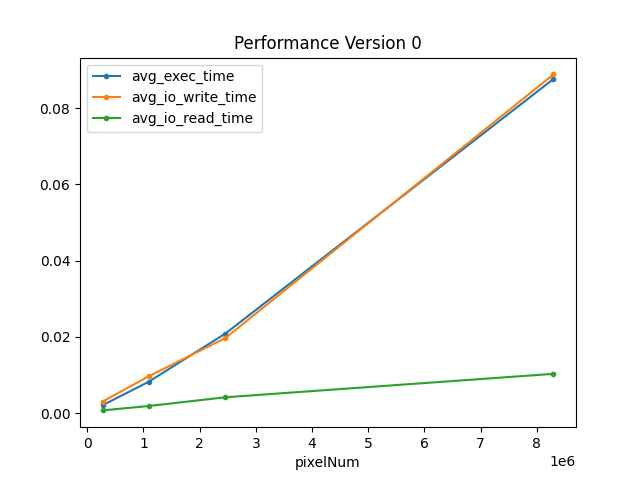
\includegraphics[width=0.5\columnwidth]{graphics/performance_vergleich}
    \caption{Performanz der Vergleichsimplementierung}
    \label{fig:performanz}
\end{figure}
Da die Vergleichsimplementierung schlicht die mathematische Definition des Verfahrens in C-Code übersetzen soll, wurden etwaige Verbesserungen wie Speicherzugriffsoptimierungen außenvor gelassen.
Die Daten des Bildes liegen Zeile für Zeile im Speicher, wobei die mathematische Definition über die einzelnen Spalten funktioniert.
Diese (kleine) Optimierung würde die Laufzeit der Vergleichsimplementierung um Faktor 2 beschleunigen, da dadurch Cachemisses signifikant reduziert werden können, aufgrund der Einfachheit, die diese Version mit sich bringen soll, wurde darauf jedoch verzichtet.
\begin{figure}[H]
    \centering
    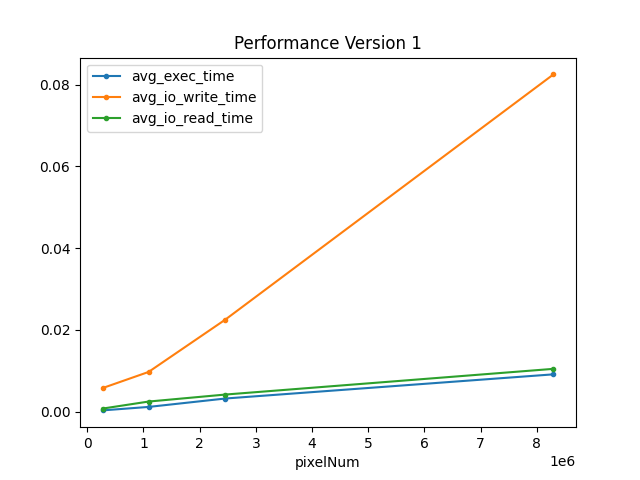
\includegraphics[width=0.5\columnwidth]{graphics/performance_simd}
    \caption{Performanz der SIMD-Implementierung}
    \label{fig:performanz-simd}
\end{figure}
Die SIMD-Implementierung erzielt in Relation zur Vergleichsimplementierung einen Speedup von circa 10.
Dies ist darauf zurückzuführen, dass zum einen die Berechnung der Sobel-Werte vektorisiert zum anderen aber auch die Speicherzugriffe optimiert werden (zeilenweiser statt spaltenweiser Zugriff).
Durch die Vektorisierung können 16 Farbchannel gleichzeitig verarbeitet werden, im Gegensatz zu der vollständig sequentiellen Berechnung der Vergleichsimplementierung.
Basierend auf dieser Information wäre der theoretisch maximale Speedup 16, was jedoch vom gemessenen Speedup von x10 abweicht, was wiederum auf den durch das versetzte Laden und aufbereiten der Vektoren entstehenden Overhead zurückzuführen ist.
Auf Assembly-Ebene entspricht dieser Overhead fast der Hälfte der Instruktionen, die für die vektorisierte Berechnung ausgeführt werden.
Optimiert man die Speicherzugriffe der Vergleichsimplementierung, kann GCC ab Optimierungsstufe 3 interessanterweise die hohe Vektorisierbarkeit des Problems eigenständig erkennen und übersetzt diese ebenfalls in Vektorinstruktionen.
Da der durch GCC generierte Ansatz jedoch nur 8 Byte gleichzeitig verarbeiten kann, ist unsere SIMD-Implementierung immer noch in etwa doppelt so schnell.

Die Threading-Implementierung kann durch ihren noch paralleleren Ansatz gegenüber der SIMD-Implementierung eine noch bessere Laufzeit mit einem theoretisch unendlichen Speedup erzielen.
Da unsere Messungen ergeben haben, dass die optimale Anzahl an Streifen, in die das Bild aufgeteilt werden soll, den durch die CPU bereitgestellten Threads entspricht, kann der Speedup (theoretisch) durch Hinzufügen beliebig vieler Kerne beliebig groß werden.
Dadurch, dass jeder Thread in der Theorie genau einen Streifen bearbeiten kann, kann die Parallelität von modernen CPUs bestmöglich ausgenutzt werden, während der Overhead für die Verwaltung der Threads möglichst gering bleibt.
Der maximal zu erwartende Speedup gegenüber der Single-Thread-SIMD-Implementierung entspricht also der Anzahl der durch die CPU bereitgestellten Threads.
Da jedoch üblicherweise nicht alle Threads dieselbe Rechenleistung liefern können, bzw.\ das Programm aufgrund des Schedulers nicht zu allen Zeitpunkten vollständig parallel arbeiten kann, weicht der gemessene Speedup stark vom theoretischen Maximum ab.
Des Weiteren ist es wichtig anzumerken, dass für besonders kleine Bilder die Threading-Implementierung - aufgrund des Thread-Verwaltungsoverheads - langsamer als die SIMD-Implementierung sein kann.

Bei der Rechereche zum Sobel-Operator fiel auf, dass so gut wie jede Implementierung Graustufenbilder zur Berechnung verwendet.
Deswegen wurden alle drei Versionen auch für Graustufenbilder implementiert.
(Bilder mit Performance)
Es zeigt sich, dass die Ausführungszeit auf den Graustufenbildern rund 1/3 der Ausführungszeit auf Farbbildern beträgt.
Somit wäre die Beschränkung auf Graustufenbilder ein einfacher Weg um eine signifikante Optimierung der Ausführungszeit zu erreichen.
Des Weiteren leidet die Kantenerkennung unter dem Fehlen der Farbe nicht, die Kanten sogar besser zu erkennen.

(2 Bilder mit Kante Farbe Kante grau)

Dies erklärt, warum so gut wie jede Impelementierung Graustufenbilder zur Berechnung benutzt.

Wie in der Einleitung bereits erwähnt, wird die Berechnung der Sobel-Werte normalerweise auf Graustufenbildern durchgeführt, da das die weitere Verarbeitung der erkannten Kanten erleichtert.
Durch diesen de-facto-Industriestandard produzieren die zusätzlichen Versionen (3-5) analog zu den Versionen 0-2 Graustufenbilder.
Da hierbei jedoch der einzige Unterschied die Pixelbreite - nämlich 8, statt 24 Bit - ist, entspricht der erwartete Speedup von 24/8 = 3 gegenüber der entsprechenden 24-Bit Implementierung genau dem gemessenen.
\section{Zusammenfassung und Ausblick}
\label{sec:zusammenfassung}
Der Sobel-Filter ist eine gängige Methode, um effizient Kanten in Bildern zu erkennen.
Er funktioniert, indem die vertikalen und horizontalen Kanten eines Bildes mit einer Matrix berechnet und anschließend zusammengefügt werden.
%Dabei ist sein Hauptanwendungsgebiet die Computer-Vision, er wird aber bspw. auch in der Medizin verwendet, um die Sichtbarkeit von Tumoren in MRT-Aufnahmen zu verbessern.
Wir haben in insgesamt 6 verschiedenen Versionen die Berechnung des Sobel-Filters implementiert und deren Laufzeiten ausgiebig analysiert.
Während Version 0 schlicht die mathematische Definition des Filters in C-Code übersetzt, verwendet Version 1 ausgeklügelte Methoden, um mit SIMD-Instruktionen mehr als 5 Pixel simultan zu berechnen.
Version 2 wiederum bringt diese Parallelität auf ein komplett anderes Niveau, indem es alle Vorteile von Version 1 mittels Multithreading mit der hohen Parallelität von modernen Rechenkernen kombiniert.
Die Versionen 3 bis 5 funktionieren gleich wie Versionen 0 bis 2 respektive, arbeiten dagegen aber auf Graustufenbildern, die in der Kantenerkennung nicht nur der de-facto Industriestandard sind, sondern eine 3-mal geringere Pixelbreite aufweisen und damit auch verlässlich dreimal so schnell abgearbeitet werden können, um selbst Bilder jenseits von 4K in wenigen Sekundenbruchteilen zu berechnen.

Ausblickend lässt sich sagen, dass eine weitere Optimierung, die bei der Arbeit mit Bildmaterial natürlich naheläge, jedoch leider den Rahmen gesprengt hätte, die Verwendung von Grafikkarten wäre.
Da unsere Implementierungen Einzelbilder jedoch problemlos sehr schnell berechnen können, würden durch die dadurch gewonnene Parallelität vor allem Video- und Echtzeitanwendungen profitieren.

% TODO: Fuegen Sie Ihre Quellen der Datei Ausarbeitung.bib hinzu
% Referenzieren Sie diese dann mit \cite{}.
% Beispiel: CR7 ist ein portugiesischer Fußballspieler ~\cite{intel2017man}.
\bibliographystyle{plain}
\bibliography{Ausarbeitung}
\end{document}